
\subsection{Grafische Oberfläche}

\subsubsection{Aufgaben}
Die dritte Komponente dieser Diplomarbeit stellt eine Anwendung dar, die ein simples Verwenden der API Funktionen ermöglichen soll. Weiters soll sie Roboterbewegungen visuell darstellen können, da nicht jeder Arbeitsplatz über ein physikalisches Robotermodell verfügt. Die Bedienung der Anwendung soll so simpel wie möglich gestaltet werden und neben diversen Einstellungsmöglichkeiten auch ein Handbuch mit detaillierten Informationen über die, im Hintergrund ablaufenden, Prozesse des Systems bieten.
\subsubsection{Aufbau}
Der Aktionsbereich der Anwendung basiert auf einem Tab-Control, wie es auch aus vielen Internet-Browsern bekannt ist. Die vier Tabs stellen zugleich die verschiedenen Anwendungsmöglichkeiten der Software dar. Im rechten Drittel der Oberfläche befindet sich die Visualisierung, welche zu jeder Zeit die Bewegsabläufe des Roboters darstellen. \\
Im oberen Bereich der Anwendung befindet sich eine Menü- und eine Werkzeugleiste, welche grundsätzliche Befehle wie Neu, Öffen und Speichern enthält. Um die Ausgabe von Eingabefehlern zu ermöglichen befindet sich eine Konsole in der unteren Sektion der Oberfläche.
\subsubsection{Umsetzung}
Wie bereits erwähnt besteht der Aktionsbereich aus dem WPF TabControl mit vier Tabs. Die Visualisierungen sind jeweils als UserControls realisiert und in eine ViewBox eingebettet. Letztere skaliert ihren Inhalt gleichmäßig, je nachdem wie groß die gesamte Oberfläche ist. Bei der Konsole handelt es sich um eine nicht editierbare Textbox auf die nur aus der Anwendung heraus Text ausgegeben wird. \\
Die Werkzeugleiste wurde mit einem sogenannten ToolBarTray realisiert und enthält eine Menge an Buttons, deren Funktionen im Kapitel "Bedienung" näher beschrieben werden. Auch die verschiedenen Menüs wurden mit Hilfe eines von WPF zur Verfügung gestellten Controls, dem Menu beziehungsweise MenuItem, in einer MenuBar realisiert.
\subsubsection{Bedienung}
\begin{figure}[H]
  \centering
  \begin{minipage}[t]{16 cm}
  	\centering
  	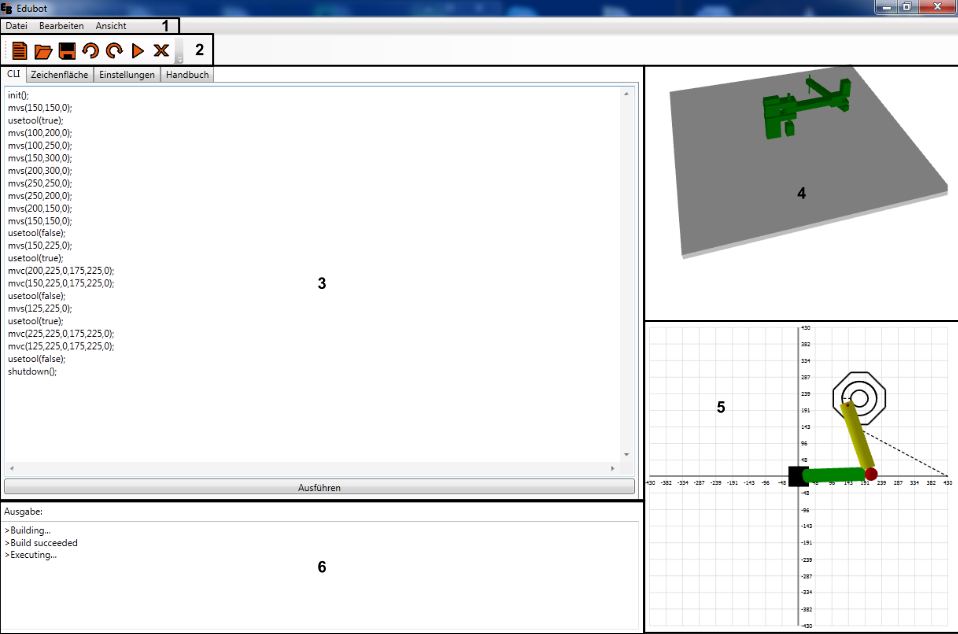
\includegraphics[width=16cm]{images/GUI} 
    \caption{Benutzeroberfläche}
  \end{minipage}
\end{figure}
\textbf{1) Menüleiste}\\
Die Menüleiste beinhaltet die drei Menüs "'Datei"', "'Bearbeiten"' und "'Ansicht"', welche über einen Klick aufgerufen werden.
\begin{itemize}
\item Datei
\begin{itemize}
\item Neu - Erstellt ein neues Skript in der Kommandozeile.
\item Öffnen - Öffnet ein vorhandenes Skript in der Kommandozeile.
\item Speichern - Speichert das aktuell geöffnete Skript. Ist keine Skript geöffnet, so wird der "'Speichern unter"'-Dialog geöffnet.
\item Speichern unter - Speichert den Inhalt der Kommandozeile in einer Textdabei mit dem angegebenen Namen.
\item Beenden - Beendet die Edubot-Anwendung.
\end{itemize}
\item Bearbeiten
\begin{itemize}
\item Rückgängig - Macht die gerade durchgeführte Aktion rückgängig (Kommandozeile oder Zeichenfläche)
\item Wiederholen - Wiederholt ein rückgängig gemachte Aktion (Kommandozeile oder Zeichenfläche)
\item Ausschneiden - Schneidet den ausgewählten Bereich aus und legt ihn in die Zwischenablage 
\item Kopieren - Kopiert den ausgewählten Bereich und legt ihn in die Zwischenablage
\item Einfügen - Fügt den Inhalt der Zwischenablage in die Kommandozeile ein
\end{itemize}
\item Ansicht
\begin{itemize}
\item Kommandozeile - Öffnet den Kommandozeile-Tab
\item Zeichenfläche - Öffnet den Zeichenfläche-Tab
\item Einstellungen - Öffnet den Einstellungen-Tab
\item Handbuch - Öffnet den Handbuch-Tab
\end{itemize}
\end{itemize}
\textbf{2) Werkzeugleiste}\\
Die Werkzeugleiste beinhaltet die wichtigsten Standardbefehle sowie weitere, anwendungsspezifische Befehle. Diese können über einen Klick auf das entsprechende Symbol ausgeführt werden.
\begin{itemize}
\item Neu - Erstellt ein neues Skript in der Kommandozeile.
\item Öffnen - Öffnet ein vorhandenes Skript in der Kommandozeile.
\item Speichern - Speichert das aktuell geöffnete Skript. Ist keine Skript geöffnet, so wird der "'Speichern unter"'-Dialog geöffnet.
\item Rückgängig - Macht die gerade durchgeführte Aktion rückgängig (Kommandozeile oder Zeichenfläche)
\item Wiederholen - Wiederholt ein rückgängig gemachte Aktion  (Kommandozeile oder Zeichenfläche)
\item Ausführen - Übersetzt die aktuell eingegebenen Befehle (Kommandozeile oder Zeichenfläche) und führt diese aus.
\item Abbrechen - Bricht die Ausführung von Befehlen durch den Roboter ab.
\end{itemize}
\textbf{3) Aktionsbereich}\\
Im Aktionsbereich findet die eigentliche Bedienung der Anwendung statt. Die verschiedenen Bereiche können über einen Klick auf den entsprechenden Tab oder den entsprechenden Eintrag im "'Ansciht"'-Menü ausgewählt werden. Eine detaillierte Beschreibung über die Bedienung der einzelnen Bereiche findet sich in den folgenden Kapiteln.\\
\textbf{4) 3D-Visualisierung}\\
Stellt die Roboterbewegungen anhand eines 3D-Modells dar, wobei zwischen einem Standard-Modell und dem Edubot-Modell gewählt werden kann. Die Auswahl is über den "Einstellungen"-Tab möglich.\\
\textbf{5) 2D-Visualisierung}\\
Stellt die Roboterbewegungen anhand eines 2D-Modells dar. Neben der Animation kann bei dieser Ansicht ein beschriftetes Koordinatensystem sowie der gefahrene Pfad betrachtet werden.\\
\textbf{6) Konsole}\\
Die Konsole gibt Informationen über potentielle Fehler bei  der Übersetzung beziehungsweise Ausführung aus. Mit Hilfe dieser Informationen können Fehler im Skript beziehungsweise ungültige Pfade behoben werden. Der Inhalt der Konsole wird bei einem Klick auf "'Ausführen"' gelöscht.
